%Copyright 2014 Jean-Philippe Eisenbarth
%This program is free software: you can 
%redistribute it and/or modify it under the terms of the GNU General Public 
%License as published by the Free Software Foundation, either version 3 of the 
%License, or (at your option) any later version.
%This program is distributed in the hope that it will be useful,but WITHOUT ANY 
%WARRANTY; without even the implied warranty of MERCHANTABILITY or FITNESS FOR A 
%PARTICULAR PURPOSE. See the GNU General Public License for more details.
%You should have received a copy of the GNU General Public License along with 
%this program.  If not, see <http://www.gnu.org/licenses/>.

%Based on the code of Yiannis Lazarides
%http://tex.stackexchange.com/questions/42602/software-requirements-specification-with-latex
%http://tex.stackexchange.com/users/963/yiannis-lazarides
%Also based on the template of Karl E. Wiegers
%http://www.se.rit.edu/~emad/teaching/slides/srs_template_sep14.pdf
%http://karlwiegers.com
\documentclass{scrreprt}
\usepackage{listings}
\usepackage{underscore}
\usepackage[bookmarks=true]{hyperref}
\usepackage[utf8]{inputenc}
\usepackage[english]{babel}
\usepackage{graphicx}
\usepackage{placeins}
\graphicspath{ {images/} }
\hypersetup{
    bookmarks=false,    % show bookmarks bar?
    pdftitle={Software Requirement Specification},    % title
    pdfauthor={Jean-Philippe Eisenbarth},                     % author
    pdfsubject={TeX and LaTeX},                        % subject of the document
    pdfkeywords={TeX, LaTeX, graphics, images}, % list of keywords
    colorlinks=true,       % false: boxed links; true: colored links
    linkcolor=blue,       % color of internal links
    citecolor=black,       % color of links to bibliography
    filecolor=black,        % color of file links
    urlcolor=purple,        % color of external links
    linktoc=page            % only page is linked
}%
\def\myversion{1.0 }
\date{}
%\title
\usepackage{hyperref}
\begin{document}

\begin{flushright}
    \rule{16cm}{5pt}\vskip1cm
    \begin{bfseries}
        \Huge{Software Testing \\and\\ Quality Assurance} \\
        \vspace{1.9cm}
        for\\
        \vspace{1.9cm}
        $Test plan$\\
        \vspace{1.9cm}
        \LARGE{Version \myversion approved}\\
        \vspace{1.9cm}
        Prepared by Wiktor Bednarek\\
        \vspace{1.9cm}
        Cranfield University\\
        \vspace{1.9cm}
        \today\\
    \end{bfseries}
\end{flushright}

\tableofcontents


\chapter*{Revision History}

\begin{center}
    \begin{tabular}{|c|c|c|c|}
        \hline
	    Name & Date & Reason For Changes & Version\\
        \hline
	    1 & 30.12.16 & update & 1.0\\
        \hline
	    2 & 30.12.16 & update & 1.1\\
        \hline
    \end{tabular}
\end{center}
\FloatBarrier
\chapter{OVERVIEW}

\section{PRODUCT NAME}


Supercomputer simulation software.

\section{PRODUCT REVISION}
Computer job is to calculate demanded  by users jobs. There are three groups of users: IT support, Researches and Students. Computer have to me efficient and working stably, reliably, without errors as well. System going to be tested in order to assure that computer will provide highest possible results quality and precisions of calculations.




\section{PRODUCT OVERVIEW}

Product was designed as completely new supercomputer solution, not upgrade or replacement. This system has been developed for complex computation like: aerodynamic computation, physics, complex math equation and advanced computer graphics.

\section{Tracking system in use}
In this project git control version system has been used.
Regular commits helps to avoid unexpected cases e.g. when whole project is deleted by an accident. Sometimes after commit some things might be changes for worse, so in that cases is nessesry to look at previous commit.


\chapter{TESTING SYNOPSIS}

\section{Items to be tested}

To be acquainted with product please look at following UML diagram:
\begin{figure}[h!]
\centering
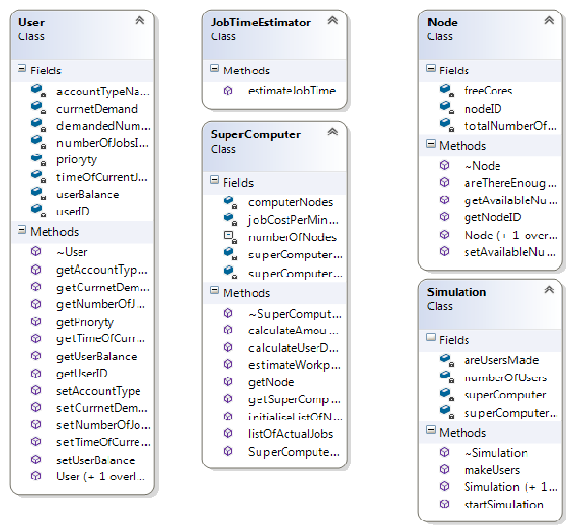
\includegraphics{ClassDiagram.png}
\caption{SuperComputer UML diagram}

\end{figure}
\FloatBarrier

\textbf{Function output to test:}

\textit{SuperComputer class}
\\
\\
void calculateUserDemandCost();
\\
Need to check whenever user demand cost is correct
\\
\\
void estimateWorkperiod(User user);
\\
Is estimated job time resuls is close to expectations?
\\
\\
double getSuperComputerIncome() const;
Is is income for specific conditions equals to expectation value?
\\
\\
void calculateAmountOfResourcesToUse(User user);
\\


\textit{User class}:
\\
\\
double getUserBalance() const;
\\
\\
    unsigned int getNumberOfJobsInQueue() const; \\
    Are there right amount of users, not to much - more than resources or to less - lower than zero
\\
\\
    void setUserBalance(double userBalance);\\
    Need to check whenever current user balance is correct
\\
\\



\textit{
JobTimeEstimator class} :
\\
\\
static double estimateJobTime(int jobType);\\
Is job times is estimated according to expectations?
  \\
 \\


\textit{Simulation class}:  
\\
\\
 void makeUsers();
 \\
 \\
 \textit{
Node class} :  
 \\
 \\
 int getAvailableNumberOfCoresInNode();\\
 Is this value is equal to expectations?
\\
\\
bool areThereEnoughFreeCores(unsigned int numberOfCoresToCheck);\\
Is this value is equal to expectations? What if number of cores less than zero?





\section{Items 
not to be Tested}



\textit{SuperComputer class}
\\
\\
void initialiseListOfNodes();
\\
\\
void listOfActualJobs();
Simple value listing
\\
\\



\textit{User class}:
\\
\\
void setAccountType(int accountTypeNum);\\
Only setting class value
\\
\\
    const std::string getAccountTypeName() const;  \\
    Only reading an value
\\
\\
     int getPrioryty() const;  \\
     Only reading an value
\\
\\
  void setNumberOfJobsInQueue(unsigned int numberOfJobsInQueue);\\
  Only setting class value
\\
\\
   unsigned int getCurrnetDemand() const;\\
    Only reading an value
\\
\\
   double getTimeOfCurrentJob() const;\\
   Only reading an value
\\
\\
void setTimeOfCurrentJob(double timeOfCurrentJob);\\
Only setting class value
\\
\\
int getUserID() const;\\
 Only reading an value
\\
\\
    void setCurrnetDemand(unsigned int currnetDemandNumber);\\
    Simple value setting function. It is not necessary to check
\\
\\
 

 \textit{
Simulation class} :  
 \\
 \\
void startSimulation();\\
This function starts another methods, however those methods itself need to be tested
 \\
 \\
 \textit{
Node class} :  
 \\
 \\
 int getAvailableNumberOfCoresInNode();\\
 Only reading an value
\\
\\
 int getNodeID();\\
 Only reading an value
 \\
 \\






\chapter{Types of testing}

In this supercomputer project Goggle Test was used for testing purpose. It provides couple simple in use but relay solid testing functions. 

\section{ACCEPTANCE TESTING}
Before test starts couple conditions has to be fulfilled.

\begin{itemize}
\item Supercomputer has to be turn on
\item Users must be created
\item Users balance has to be above 0 
(it is relay unlikely since balance is  setted by default on initialization list before object instance of User class is created).
\item  Supercomputer Nodes have to initialised
\end{itemize} 



\section{FEATURE LEVEL TESTING}


\subsection{Boundary Tests}

\begin{itemize}
\item SuperComputer function getUserBalance(). Need to check whenever user balance in not smaller than zero, as well it is not exceeding ) integer scope.
\item SuperComputer function estimateWorkperiod(). Need to check whenever period in not smaller than zero, as well it is not exceeding  integer scope.
\item SuperComputer function gcalculateUserDemandCost(). Need to check whenever cost of job selected by user is in not smaller than zero, as well it is not exceeding integer scope.
\\
\textbf{\item Generally all getter functions in this project have to be checked whenever function return value is in not smaller than zero, as well it is not exceeding integer scope.}
\end{itemize} 


\subsection{Task-Oriented Functional Tests }

\begin{itemize}
\item SuperComputer function getComputerIncomee(). Need to check whenever income is non smaller or higher than expected value e.g. ASSERT_FLOAT_EQ(actual, expected) returns true for specified: number of users, each job cost, each user initial balance, so that expected income is easy to calculate manually. 
\\
\textbf{\item Generally in all Task-Oriented Functional Tests is needed to check whenever output value is non less or higher than expected value e.g. ASSERT_FLOAT_EQ(actual, expected) returns true for specified: number of users, each job cost, each user initial balance, so that expected value is easy to calculate manually. }
\end{itemize} 


\chapter{TEST SCHEDULE AND RESOURCES}



\section{Appendix A: Glossary}


\section{Appendix B: Analysis Models}


\section{Appendix C: To Be Determined List}


\end{document}
